	\documentclass[a4paper,12pt]{article} % тип документа
%  Русский язык
\usepackage[warn]{mathtext}
\usepackage[T2A]{fontenc}			% кодировка
\usepackage[utf8]{inputenc}			% кодировка исходного текста
\usepackage[english,russian]{babel}	% локализация и переносы
% Математика
\usepackage{amsmath,amsfonts,amssymb,amsthm,mathtools} 
\usepackage{wasysym}
%%%
\usepackage{graphicx}



\begin{document}
%титул
\hrule 
\medskip
\begin{raggedright}
{\large \textbf{Отсчёт по работе 1.1.4}}
\\
\medskip
{\Large Измерение интенсивности радиационного фона} 
\\
\medskip
{\large Карташов Констанин Б04-005}
\medskip
\hrule
\medskip
\end{raggedright}


\section{Обобщение}

Целью работы является применение методов обработки экспериментальных данных для изучения статистических закономерностей при измерении интенсивности радиационного фона. Для измерений используется счётчик Мюллера-Гейгера, подключённый к компьютеру. Компьютер проводит 400 измерений длительностью в 10 секунд, фиксируя количество срабатываний счётчика за время одного измерения. После проведения измерений компьютер выводит статистические данные для 400 измерений длительностью в 10 секунд и количественные данные для 200 измерений длительностью в 20 секунд. Затем из данных для измерений в 20 секунд следует вывести статистические данные и проанализировать статистические данные для измерений в 10 и в 20 секунд. Результатом работы является $13,73\pm0,18$ частиц в среднем для измерений в 10 секунд и $27,48\pm0,36$ для измерений в 20 секнд.
\medskip\hrule\medskip

\section{Теоретическая часть}

Радиационный фон состоит в основном из космических лучей прилетающих из Галактики и частиц возникающих при взаимодействии первых с атмосферой Земли. При прохождении таких частиц через счётчик Гейгера-Мюллера (далее - счётчик), счётчик генерирует короткие электрические импульсы, которые в этой работе будет фиксироваться при помощи компьютера.\\

Прохождение космических через счётчик – пуассоновский процесс. Для такого процесса среднеквадратичная ошибка числа обсчётов, измеренное за некоторый интервал времени равна квадратному корню из среднего числа отсчетов $ n_0 $ за тот же интервал: $ \sigma= \sqrt{n_0} $. однако истинное среднее значение измеряемой величины неизвестно. поэтому в формулу для определения стандартной ошибки отдельного измерения приходится подставляет не истинное среднее значение $ n_0 $ , а  измеренное значение $ n $:
\begin{equation}
\sigma = \sqrt{n}
\end{equation}

Из формулы (1) следует, что, с вероятностью 68\%, измеренное число частиц $n$ отличается от искомого среднего не более чем на $ \sqrt{n} $. Результат измерения записывается вот так:
\begin{equation}
n_0 = n \pm \sqrt{n}
\end{equation}

При $ N $ измерениях среднее значеие числа сосчитаных за одно измерение частиц равно:
\begin{equation}
\bar{n}=\frac{1}{N} \sum_{i=1}^{N} n_i
\end{equation}

Стандартную ошибку отдельного измерения можно оценить по следущей формуле:
\begin{equation}
\sigma_{отд} = \sqrt{\frac{1}{N}\sum_{i=1}^{N} \left( n_i - \bar{n} \right)^2}
\end{equation}

В соответствии с формулой (1) следует ожидать, что эта ошибка будет близка к $ \sqrt{n_i} $, т. е. $ \sigma_{отд} \approx \sigma_i = \sqrt{n_i} $, где в качестве $ n_i $ можно подставить любое из измеренных значений $ n $. Ближе всего к значению $ \sigma_{отд} $, определённому по формуле (4), лежит величина $ \sqrt{\bar{n}} $, т. е.
\begin{equation}
\sigma_{отд} \approx \sqrt{\bar{n}}
\end{equation}

Величина $ \bar{n} $ из формулы (3), полученная путём усреднения резутатов по серии из $ N $ опытов сама является случайной величиной, для которой можно посчитать стандартную ошибку отклонения $ \bar{n} $ от $ n_0 $:
\begin{equation}
\sigma_{\bar{n}}=\frac{1}{N}\sqrt{\sum_{i=1}^{N} \left( n_i - \bar{n} \right)^2} = \frac{\sigma_{отд}}{\sqrt{N}}
\end{equation}

Аналогичным образом определяется относительная ошибка в определении среднего по всем измерения значения $\bar{n}$:
\begin{equation}
\varepsilon_{\bar{n}}=\frac{\sigma_{\bar{n}}}{\bar{n}}=\frac{\sigma_{отд}}{\bar{n}\sqrt{N}} \approx \frac{1}{\sqrt{\bar{n}N}}.
\end{equation}

\medskip\hrule\medskip

\section{Экспериментальная часть}

1. Включаем компьютер и проводим измерения.

2. После измерений следующие данные были вычислены компьютером(значения полученные для измерений длительностью в 10 секунд будут обозначатся с индексом $X_1$, для измерений в 20 секунд  с индексом $ X_2 $):

\[ \bar{n}_1 = 13,73; \;\;\; \sigma_{\bar{n}_1} = 0,181384; \;\;\; \varepsilon_{\bar{n}_1} = 1,32107; \;\;\; \sigma_1 = 3,62767.    \]


3. Также компьютером подсчитано, что в пределах $ \pm \sigma_1 $ находится 67,9\% измерений, а в пределах $ \pm 2\sigma_1 $ находится 92,6\% измерений.

4. Получим окончательный результат для измерений за 20 с
\[ n_{t=10c}=\bar{n}_1 \pm \sigma_{\bar{n}_1}=13,73\pm 0,18. \]

5. Далее компьютером была составлина следщая таблица числа срабатываний счётчика за 20 с (табл. 1)\\

\begin{table}[p]
\centering
\begin{tabular}{|l|l|l|l|l|l|l|l|l|l|l|}
\hline
№ опыта & 1  & 2  & 3  & 4  & 5  & 6  & 7  & 8  & 9  & 10 \\ \hline
0       & 38 & 27 & 26 & 36 & 34 & 27 & 25 & 22 & 26 & 26 \\
10      & 34 & 27 & 32 & 34 & 29 & 29 & 34 & 26 & 28 & 36 \\
20      & 28 & 31 & 28 & 22 & 27 & 27 & 27 & 33 & 30 & 25 \\
30      & 31 & 24 & 28 & 29 & 25 & 34 & 25 & 33 & 29 & 27 \\
40      & 35 & 31 & 30 & 22 & 30 & 24 & 19 & 31 & 23 & 43 \\
50      & 15 & 29 & 37 & 27 & 30 & 20 & 23 & 24 & 29 & 21 \\
60      & 34 & 29 & 32 & 30 & 19 & 26 & 19 & 21 & 17 & 20 \\
70      & 35 & 23 & 29 & 27 & 37 & 30 & 33 & 30 & 31 & 24 \\
80      & 26 & 33 & 17 & 27 & 29 & 23 & 24 & 34 & 22 & 17 \\
90      & 31 & 30 & 41 & 26 & 28 & 21 & 28 & 28 & 22 & 32 \\
100     & 28 & 21 & 20 & 24 & 28 & 27 & 32 & 25 & 24 & 22 \\
110     & 30 & 21 & 32 & 20 & 28 & 24 & 30 & 27 & 30 & 27 \\
120     & 25 & 25 & 29 & 34 & 33 & 28 & 26 & 23 & 29 & 26 \\
130     & 31 & 31 & 31 & 24 & 29 & 24 & 33 & 16 & 29 & 22 \\
140     & 37 & 25 & 25 & 32 & 27 & 17 & 23 & 29 & 22 & 26 \\
150     & 30 & 27 & 33 & 33 & 30 & 27 & 18 & 26 & 22 & 26 \\
160     & 26 & 28 & 28 & 19 & 30 & 29 & 25 & 25 & 24 & 25 \\
170     & 29 & 26 & 28 & 36 & 30 & 31 & 24 & 32 & 34 & 33 \\
180     & 26 & 35 & 18 & 22 & 27 & 21 & 23 & 21 & 42 & 25 \\
190     & 27 & 27 & 35 & 25 & 26 & 33 & 29 & 22 & 21 & 29 \\ \hline
\end{tabular}
\caption{Число срабатываний счетчика за 10 с}
\end{table}

6. Гистограммы для распередений среднего числа отсчетов за 10 и 20 с строим на одном графике (рис. 1). При этом для второго распеределения цену деления по оси абцисс увеличивает в  раза, чтобы положения максимумов распределений совпали.
\begin{figure}[p]
\centering
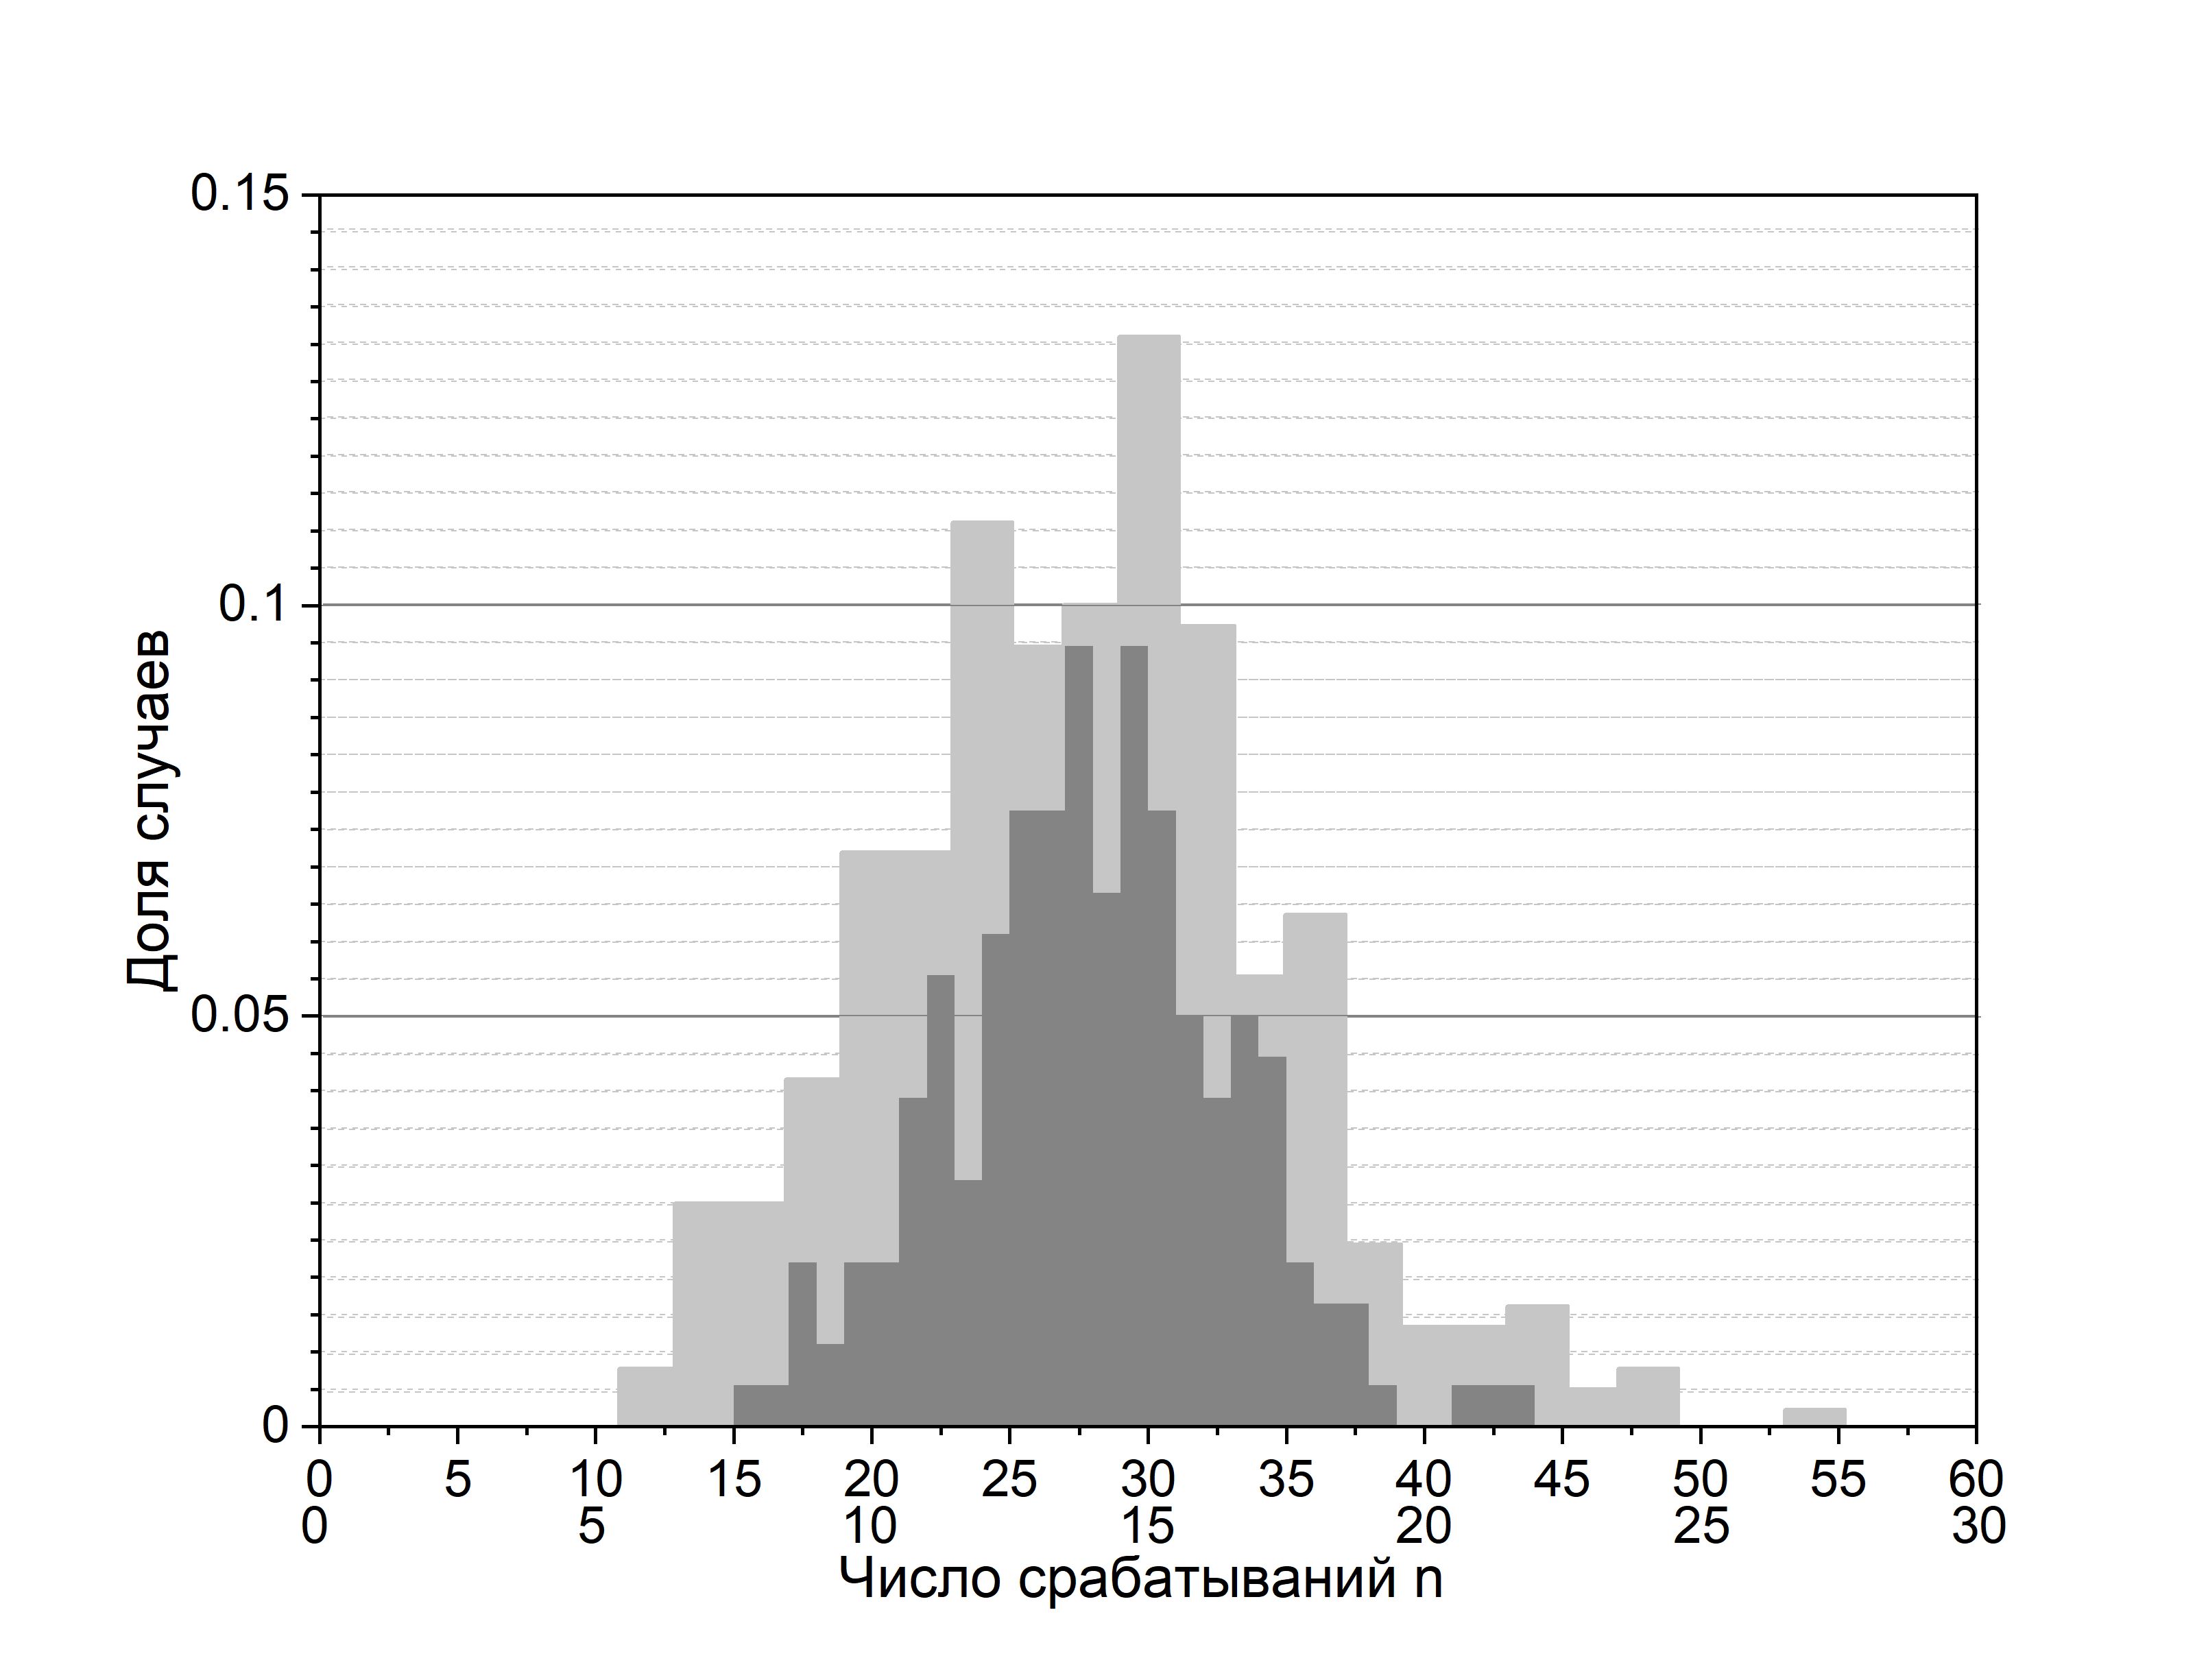
\includegraphics[width=15cm]{Graph1.png}
\caption{Гистограммы для $\tau = 10$ c и $\tau = 20$ с}
\end{figure}


7. Используя формулу (3), опредклим среднее число импульсов счётчика за 20 с:
\[ \bar{n}_2=\frac{1}{N_2} \sum_{i=1}^{N_2} n_i = 27,475. \]

8. Найдём среднеквадратичную ошибку отдельного измерения по формуле (4):
\[  \sigma_{2} = \sqrt{\frac{1}{N_2}\sum_{i=1}^{N_2} \left( n_i - \bar{n}_2 \right)^2} \approx 5,029.  \]

9. Убедимся в справедливости формулы (5):
\[  \sigma_2 \approx \sqrt{\bar{n}_2}; \;\;\;\; 5,029 \approx \sqrt{27,475} = 5,242.\]

10. В пределах $ \pm \sigma_2 $ находится 66\% измерений, а в пределах $ \pm 2\sigma_2  $ находится 95\% измерений.

11. Сравним среднеквадратичные ошибки отдельных измерений для двух распределений: $ \bar{n}_1 = 13,73; \sigma_1 = 3,63; \bar{n}_2 =27,46; \sigma_2 = 5,03 $ . Легко видеть, что хотя абсолютное значение сигма во втором распределении больше, чем в первом, относительная полуширина второго распределения меньше:
\[  \frac{\sigma_1}{\bar{n}_1} \cdot 100\% = 26\%; \;\;\;\; \frac{\sigma_2}{\bar{n}_2} \cdot 100\% = 18\%. \]

12. Определим стандартную ошибку для величины $ \bar{n}_2 $ и относительную ошибку нахождения $ \bar{n}_2 $ для $ N_2 = 200 $ измерений по 20 с. По формуле (6)
\[ \sigma_{\bar{n}_2} = \frac{\sigma_2}{\sqrt{N_2}}=0,356  \]
Относительная ошибка первому равенству (7):
\[ \varepsilon_{\bar{n}_2} = \frac{\sigma_{\bar{n}_2}}{\bar{n}_2} \cdot 100\% =1,29\%, \]
по второму равенству:
\[ \varepsilon_{\bar{n}_2} = \frac{100\%}{\sqrt{\bar{n}_2 N_2}} =1,35\%; \]
Окончательный результат:
\[ n_{t=20c}=\bar{n}_2 \pm \sigma_{\bar{n}_2}=27,48\pm 0,36. \]







%\[ \bar{n}_1 = 13,73 \]
%\center{\scriptsize{Среднее число частиц за 1 измерение}}
%\[ \sigma_{\bar{n}_1} = 0,181384 \]
%\center{\scriptsize{Стандартная ошибка измерения среднего}}
%\[ \varepsilon_{\bar{n}_1} = 1,32107 \]
%\center{\scriptsize{Относительная ошибка измерения среднего}}

%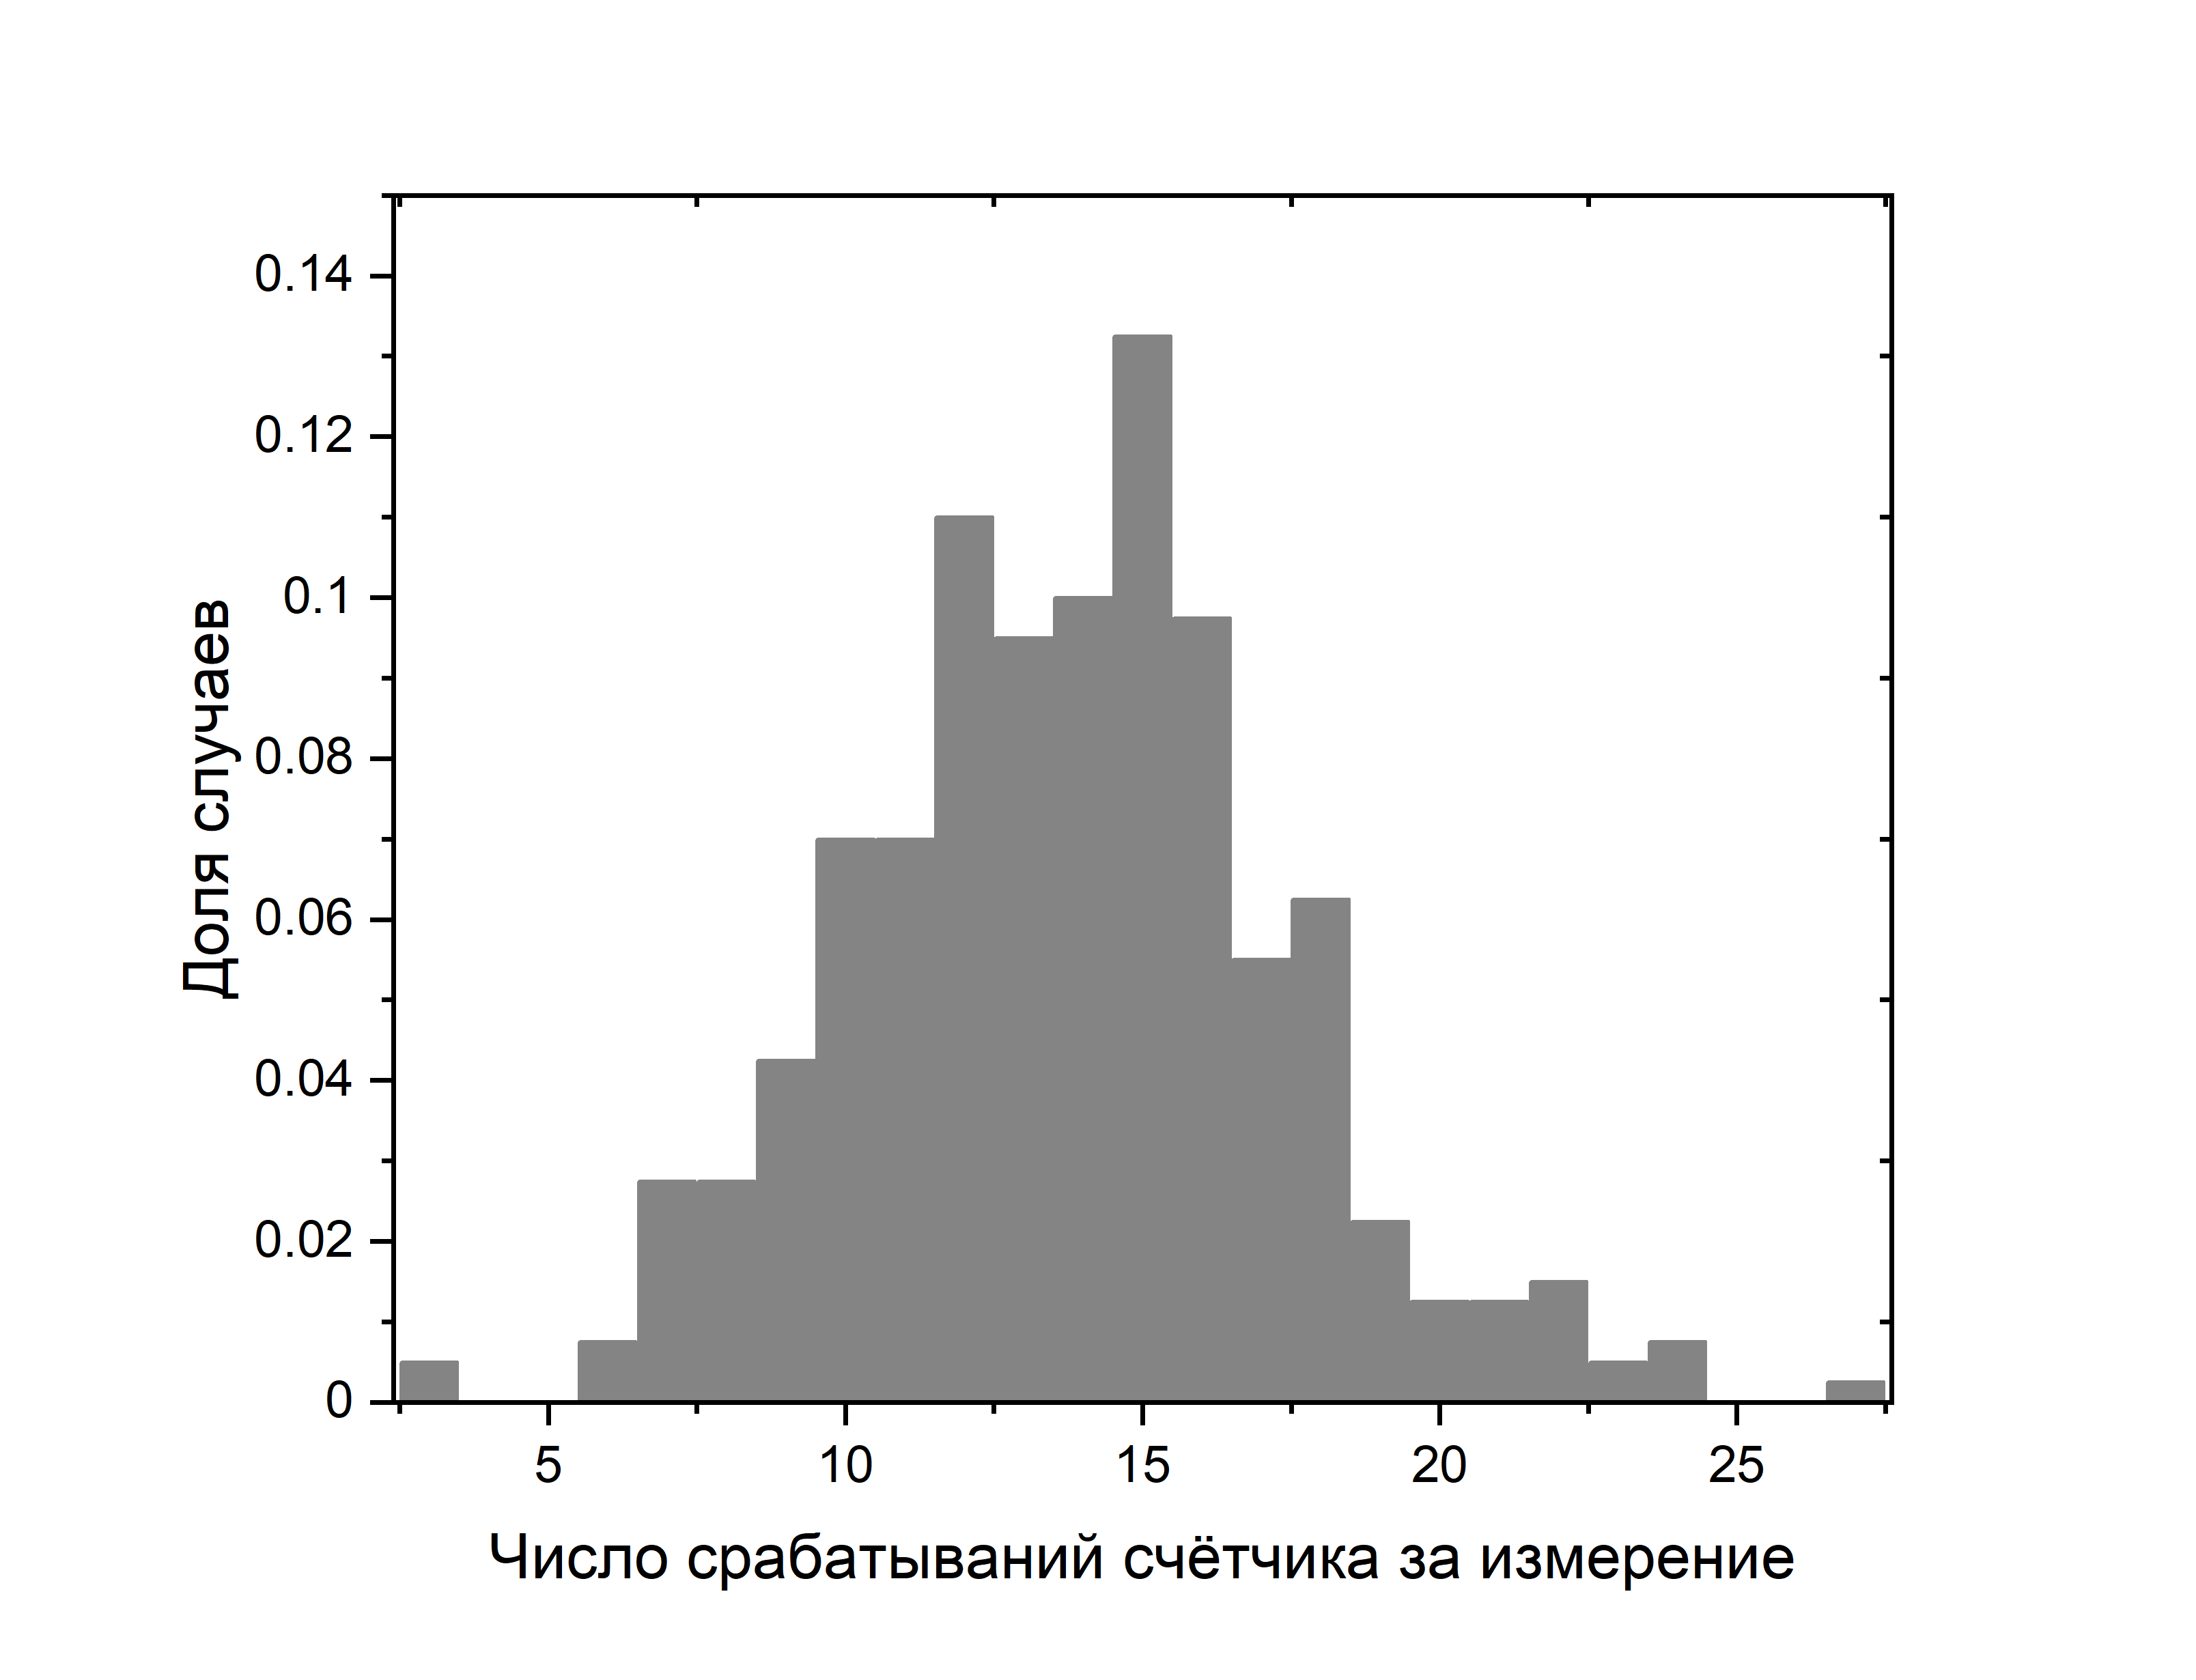
\includegraphics[width=10cm]{hist1.png}

\medskip\hrule\medskip

\section{Заключительная часть}

Проведя измерения и проанализировав полученные данные мы показали, что процесс срабатывания счётчика Гейгера-Мюллера схож с пуассоновским процессом. Также мы нашли среднее число срабатывание счётчика за период в 10 и 20 с, стандартную ошибку этих измерений, и стандартную ошибку отклонения среднего числа от действительного.\\
В таблице 2 предствлены полученные результаты.

\begin{table}[h]
\centering
\caption{Результаты работы}
\begin{tabular}{|c|c|}
\hline 
$n_{t=10c}$ & $13,73\pm 0,18$ \\ 
\hline 
$\bar{n}_1$ & $13,73$ \\ 
\hline 
$\sigma_1$ & $3,63$ \\ 
\hline 
$ \sigma_{\bar{n}_1}$ & $ 0,18 $ \\ 
\hline 
$ \varepsilon_{\bar{n}_1}$ & $ 1,32\% $ \\ 
\hline 
$n_{t=20c}$ & $13,73\pm 0,18$ \\ 
\hline 
$\bar{n}_2$ & $27,48$ \\ 
\hline 
$\sigma_2$ & $ 5,03 $\\ 
\hline 
$ \sigma_{\bar{n}_2}$ & $ 0,36  $ \\ 
\hline 
$ \varepsilon_{\bar{n}_2}$ & $1,29\%$ \\ 
\hline 
\end{tabular} 
\end{table}

\medskip\hrule\medskip

\end{document}
